%\documentclass[11pt, twocolumn]{article}
\documentclass[11pt,a4paper]{article}
%\usepackage[top=0.85in,left=2.75in,footskip=0.75in]{geometry}
\usepackage[top=1in,bottom=1in]{geometry}

% Use adjustwidth environment to exceed column width (see example table in text)
\usepackage{changepage}

% Use Unicode characters when possible
\usepackage[utf8x]{inputenc}

% textcomp package and marvosym package for additional characters
\usepackage{textcomp,marvosym}

% cite package, to clean up citations in the main text. Do not remove.
%\usepackage{cite}

% line numbers
\usepackage[right]{lineno}

% ligatures disabled
\usepackage{microtype}
\DisableLigatures[f]{encoding = *, family = * }

% color can be used to apply background shading to table cells only
\usepackage[table]{xcolor}

% array package and thick rules for tables
\usepackage{array}

% create "+" rule type for thick vertical lines
\newcolumntype{+}{!{\vrule width 2pt}}

% Bold the 'Figure #' in the caption and separate it from the title/caption with a period
% Captions will be left justified
%\usepackage[aboveskip=1pt,labelfont=bf,labelsep=period,justification=raggedright,singlelinecheck=off]{caption}
\usepackage[aboveskip=1pt,labelfont=bf,labelsep=period,singlelinecheck=off]{caption}
\renewcommand{\figurename}{Fig}

% Bibliography related
\usepackage[round,numbers,sort&compress]{natbib} 
\bibliographystyle{unsrtnat}

% Graphics
\usepackage{graphicx,color}% Include figure files
\usepackage{epstopdf}

% Misc.
%\usepackage{adjustbox}

% Math
\usepackage[intlimits]{amsmath}
\usepackage{amsfonts}
\usepackage{bm}
\usepackage{amssymb}
\usepackage{mathtools}


% Title, Authors, etc.
\title{Use case of PMF calculations in GROMACS for BioExcel}
\usepackage{authblk}

% Leave date blank
%\date{}
\author{Viveca Lindahl}

\begin{document}
\maketitle
\tableofcontents

\section{Background}
Calculating free energy (FE) differences between different conformational states is central to molecular dynamics (MD) simulation studies of biological systems. The GROMACS simulation software package is capable of carrying out efficient and highly parallel computations. However, for a large-scale study there are many technical steps on the way posing significant barriers for the non-expert user. Figure~\ref{fig:mdworkflow} shows a typical MD workflow -- using experimental data combined with modeling as input, the goal is to  make novel predictions or observations inaccessible to real-life experiments. The simulation component of the workflow has significant complexity that is currently not automated and requires time-consuming planning and management from the user. The scientific question typically involves comparing different simulation conditions, e.g. different compounds in drug discovery,different mutations in DNA and protein studies and different force field models to gauge the universality of the results,  multiplying the number of simulations (by a number $n_1$, in Fig~\ref{fig:mdworkflow}).Furthermore, the full simulation setup should be replicated in order to obtain reliable estimate of the statistical uncertainty, further multiplying the number of simulations ($n_2$).  Also, in particular for FE calculations, efficient sampling is key. For finite simulation times complex system get trapped in metastable states, yielding unreliable statitsics. However, sampling can be enhanced by advanced sampling techniques that typically exploit non-equilibrium sampling in combination with bias potentials to promote transitions between metastable states. The efficiency of such methods can further be improved by simultaneously launching multiple ($n_3$) communicating trajectories, also known as ``walkers'', that share the sampled data on-the-fly enabling more efficient extraction of information than in the case of launching the same number of independent simulations.     


\begin{figure*}[thbp!]
%\includegraphics[width=1\textwidth]{figs/config.pdf}                                                                                                           
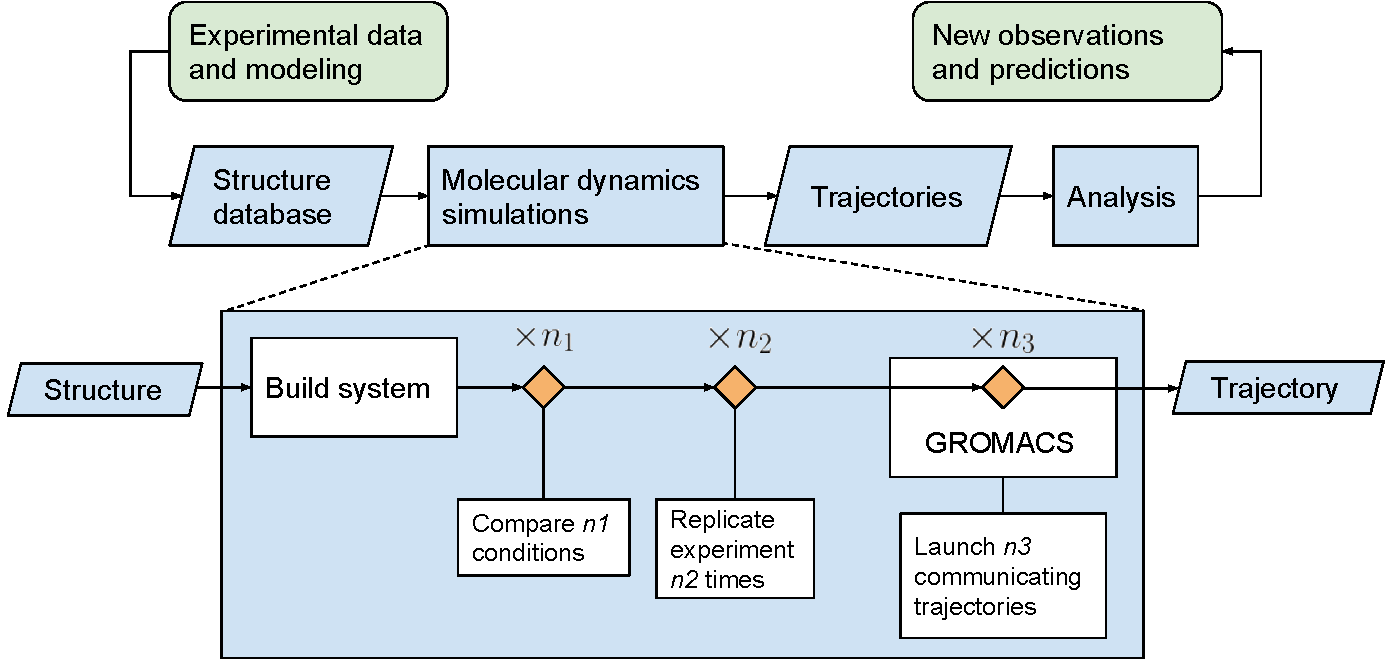
\includegraphics[width=1\textwidth]{figs/md-workflow.pdf}
\caption{\label{fig:mdworkflow}
\textbf{An MD workflow.} 
MD Simulations take experimental data and modeling (green, top-left) of complex, biomolecular sytems as input to generate trajectories that can subsequently be analyzed to extract biological insight and predictions (green, top-right). Carrying out the MD simulations can be complex in a realistc scientific application (bottom) since multiple ensembles of trajectories need to be generated (bottom). 
}
\end{figure*}
%\subsection{Challenges}

\section{Aims}
 The aim of this BioExcel project is to study and demonstrate a realistic large-scale use described below, of free energy calculations using the molecular simulation software package GROMACS. Besides serving as a tutorial or a template for the novice, this work will identify the critical components of this type of calculation, which will be helpful for designing a maximally automated procedure.case, 
%\subsection{Applicability}
\section{Methods}
Several aquaporins are in addition selectively permeable to certain solutes 


\section{Results}
\subsection{Use case I: sequence dependency of DNA base pair opening}
\subsubsection{Biological relevance and scientific aims}

\subsubsection{Methods and system setup}

\subsection{Use case II: permeability and selectivity of aquaporin membrane channel}
\subsubsection{Biological relevance and scientific aims}
\cite{lindahl2018permeability}
\subsubsection{Methods and system setup}

\section{Summary/Outlook}

\bibliography{summary}


\end{document}
